\documentclass[a4paper]{article}
\usepackage[italian]{babel}
\usepackage[italian]{isodate}  		% formato delle date in italiano
\usepackage{graphicx}				% gestione delle immagini
\usepackage{amsfonts}
\usepackage{booktabs}				% tabelle di qualità superiore
\usepackage{amsmath}				% pacchetto matematica
\usepackage{stmaryrd} 				% per '\llbracket' e '\rrbracket'
\usepackage{amsthm}					% teoremi migliorati
\usepackage{enumitem}				% gestione delle liste
\usepackage{pifont}					% pacchetto con elenchi carini

\usepackage[x11names]{xcolor}		% pacchetto colori RGB
% Link ipertestuali per l'indice
\usepackage{xcolor}
\usepackage[linkcolor=black, citecolor=blue, urlcolor=cyan]{hyperref}
\hypersetup{
	colorlinks=true
}

%\usepackage{showframe}				% visualizzazione bordi
%\usepackage{showkeys}				% visualizzazione etichetta

\begin{document}
	% indice
	\tableofcontents
	
	\newpage
	
	\section{Fondamenti}
	
	\subsection{Matematica preliminare}
	
	\subsubsection{Numeri complessi}
	
	Un numero complesso $c$ appartiene all'insieme dei complessi $\mathbb{C}$ e la sua forma è del tipo:

	\begin{equation*}
		c = \Re + j \Im
	\end{equation*}

	\noindent
	con $\Re, \Im$ variabili $\in\mathbb{R}$ e $j$ chiamata \emph{unità immaginaria} rappresentata come $j = \sqrt{-1}$. Inoltre, $\Re$ rappresenta la \emph{parte reale} e $\Im$ la \emph{parte immaginaria}. Il coniugato di $c$ è
	
	\begin{equation*}
		\tilde{c} = \Re - j \Im
	\end{equation*}

	I numeri complessi, dal punto di vista geometrico, possono essere visti come punti su un piano (chiamato \emph{piano complesso}) e descritti da coordinate $(R, I)$. Nel piano complesso, le ascisse ($x$) sono rappresentate dalla parte reale, mentre le ordinate ($y$) dalla parte immaginaria.
	
	Spesso è utile rappresentare i numeri complessi in coordinate polari formate nel seguente modo $\left(modulo, angolo\right)$. Questa forma viene denominata \emph{forma polare} di un numero complesso:
	
	\begin{equation*}
		c = \Re + j \Im = |c| (\cos{\theta} + j \sin{\theta})
	\end{equation*}

	\noindent
	dove:
	
	\begin{equation*}
		|c| = \sqrt{\Re^2 + \Im^2} \longrightarrow \text{chiamato \emph{modulo} o \emph{magnitudo}}
	\end{equation*}

	\noindent
	invece, \emph{theta} rappresenta:
	
	\begin{equation*}
		\theta \cong \arctan{\left(\dfrac{\Im}{\Re}\right)} \longrightarrow \text{chiamato \emph{angolo}, \emph{fase} o \emph{argomento \underline{in radianti}}}
	\end{equation*}

	Grazie alla formula di Eulero:
	
	\begin{equation*}
		e^{j \theta} = \cos{\theta} + j \sin{\theta}
	\end{equation*}
	
	\noindent
	è possibile riscrivere la forma polare di un numero complesso in maniera alternativa, ossia:
	
	\begin{equation*}
		c = \Re + j \Im = |c|\left(\cos{\theta} + j \sin{\theta}\right) = |c| e^{j \theta}
	\end{equation*}

	La \textbf{somma} e la \textbf{moltiplcazione} di due numeri complessi diventa:
	
	\begin{gather*}
		c_1 = R_1 + j I_1 \hspace{2em} c_2 = R_2 + j I_2 \\
		\text{Somma: } c_1 + c_2 = \left(R_1 + R_2\right) + j \left(I_1 + I_2\right) \\
		\text{Moltiplicazione con Eulero: } c_1\cdot c_2 = \left(R_1 R_2 - I_1 I_2\right) + j \left(R_1 I_2 + I_1 R_2\right) \longrightarrow = |c_1| |c_2| e^{j\left(\theta_1 + \theta_2\right)}
	\end{gather*}

	\newpage

	\subsubsection{Funzioni complesse di variabile reale}

	Dato $t \in \mathbb{R}$, una funzione $f$ complessa di variabile reale è $f: D_1 \subseteq \mathbb{R} \rightarrow D_2 \subseteq \mathbb{C}$. Viene introdotto questo concetto poiché il \textbf{\emph{fasore}} è un \underline{esempio fondamentale}. Le \textbf{caratteristiche} di questa funzione:
	
	\begin{itemize}
		\item È una funzione complessa che modella la posizione di un punto che ruota attorno all'orgiine con raggio determinato $|c|$ e velocità angolare costante $\theta{(t)}$.
		
		\item Se la funzione fosse nei numeri reali, sarebbe più dispendioso in termini di numero di funzioni da utilizzare.
	\end{itemize}
	
	L'\textbf{obbiettivo} dei fasori è quello di \emph{passare dal dominio del \underline{tempo}} (o spazio) \emph{a quello dell'\underline{analisi frequenziale}}.\newline
	La particolarità è che nel tempo il fasore riesce a variare un numero complesso (in forma polare) mantenendo il modulo $|c|$ fisso:

	\begin{equation*}
		|c| e^{j\theta} \rightarrow |c| e^{j\theta{(t)}}
	\end{equation*}

	\noindent
	dove $\theta{(t)}$ indica la \textbf{\emph{velocità angolare}}. Quest'ultima può essere calcolata tramite:
	
	\begin{equation*}
		\theta{(t)} \longrightarrow \dfrac{2\pi}{T_0} t + \phi
	\end{equation*}

	\noindent
	dove $T_0$ indica il \emph{tempo} impiegato per eseguire $2\pi$ radianti.
	
	Solitamente si utilizza il fasore con le seguenti supposizioni:
	
	\begin{itemize}
		\item[\ding{45}] Coordinate rappresentate con $(R, I)$
		\item[\ding{45}] Impostata una distanza unitaria fissa dall'origine $|c| = 1$
		\item[\ding{45}] Velocità angolare \underline{costante} pari a $2\pi/sec.$, ossia $\theta{(t)} = 2\pi t, T_0 = 1\mathrm{sec.}$
		\item[\ding{45}] Con $t = 0$ si ha $\theta = 0$
		\item[\ding{45}] Viene mantenuto $\phi = 0$
	\end{itemize}

	\newpage
	
	\subsubsection{Funzioni pari e dispari}
	
	Una funzione $f:\mathbb{R}\rightarrow\mathbb{R}$ è \textbf{\emph{pari}} se e solo se:
	
	\begin{equation*}
		f(t) = f(-t)
	\end{equation*}

	\noindent
	Invece, una funzione $f:\mathbb{R}\rightarrow\mathbb{R}$ è \textbf{\emph{dispari}} se e solo se:
	
	\begin{equation*}
		f(t) = -f(-t)
	\end{equation*}

	\newpage
	
	\subsubsection{Segnali periodici}
	
	Un segnale $f$ è \textbf{\emph{periodico}} di periodo $T$ o $T$-periodico se:
	
	\begin{equation*}
		\exists\:T_0 \in R^+ : f \left(t + T_0\right) = f(t), \hspace{1em} \forall t \in D_1
	\end{equation*}

	\noindent
	e $T_0$ è il minor numero per cui la condizione di ripetizione si verifica.
	
	Dato un periodo $T_0$ con la lettera $\mu_0$ si indica la \textbf{\emph{frequenza fondamentale}}:
	
	\begin{equation*}
		\mu_0 = \dfrac{1}{T_0}
	\end{equation*}

	Fissato $T_0 > 0$ i \textbf{\emph{segnali trigonometrici}}  di \underline{minimo periodo} $T_0$ sono:
	
	\begin{equation*}
		f(t) = \cos{\left(2 \pi \mu_{0} t \right)} \hspace{2em} f(t) = \sin{\left(2 \pi \mu_0 t\right)}
	\end{equation*}

	\noindent
	dove $\mu$ è una frequenza generale, mentre $\mu_0 = \dfrac{1}{T_0}$ è la \textbf{frequenza fondamentale}. Invece, spesso la \textbf{velocità angolare} o \textbf{\emph{pulsazione}} viene rappresentata come:
	
	\begin{equation*}
		2 \pi \mu_0 = \dfrac{2\pi}{T_0} = \omega_0
	\end{equation*}

	Inoltre, fissato un $\theta\in\mathbb{R}$ chiamato \textbf{\emph{fase}} si osserva che anche le funzioni:
	
	\begin{equation*}
		f(t) = \cos{\left(2 \pi \mu_0 t + \theta\right)} \hspace{2em} f(t) = \sin{\left(2 \pi \mu_0 t + \theta\right)}
	\end{equation*}

	\noindent
	hanno il medesimo periodo $T$.
	
	\noindent
	Infine, la fase $\theta$ permette di eseguire operazione di \emph{shift}.
	
	\newpage
	
	\subsection{Operazioni fondamentali}
	
	\subsubsection{Somma}
	
	La \textbf{\emph{somma}} di due segnali è facile quando essi non interferiscono, ovvero quando \textbf{non} sono contemporaneamente $\ne 0$. Alcuni esempi qui di seguito.
	
	\begin{figure}[!htp]
		\centering
		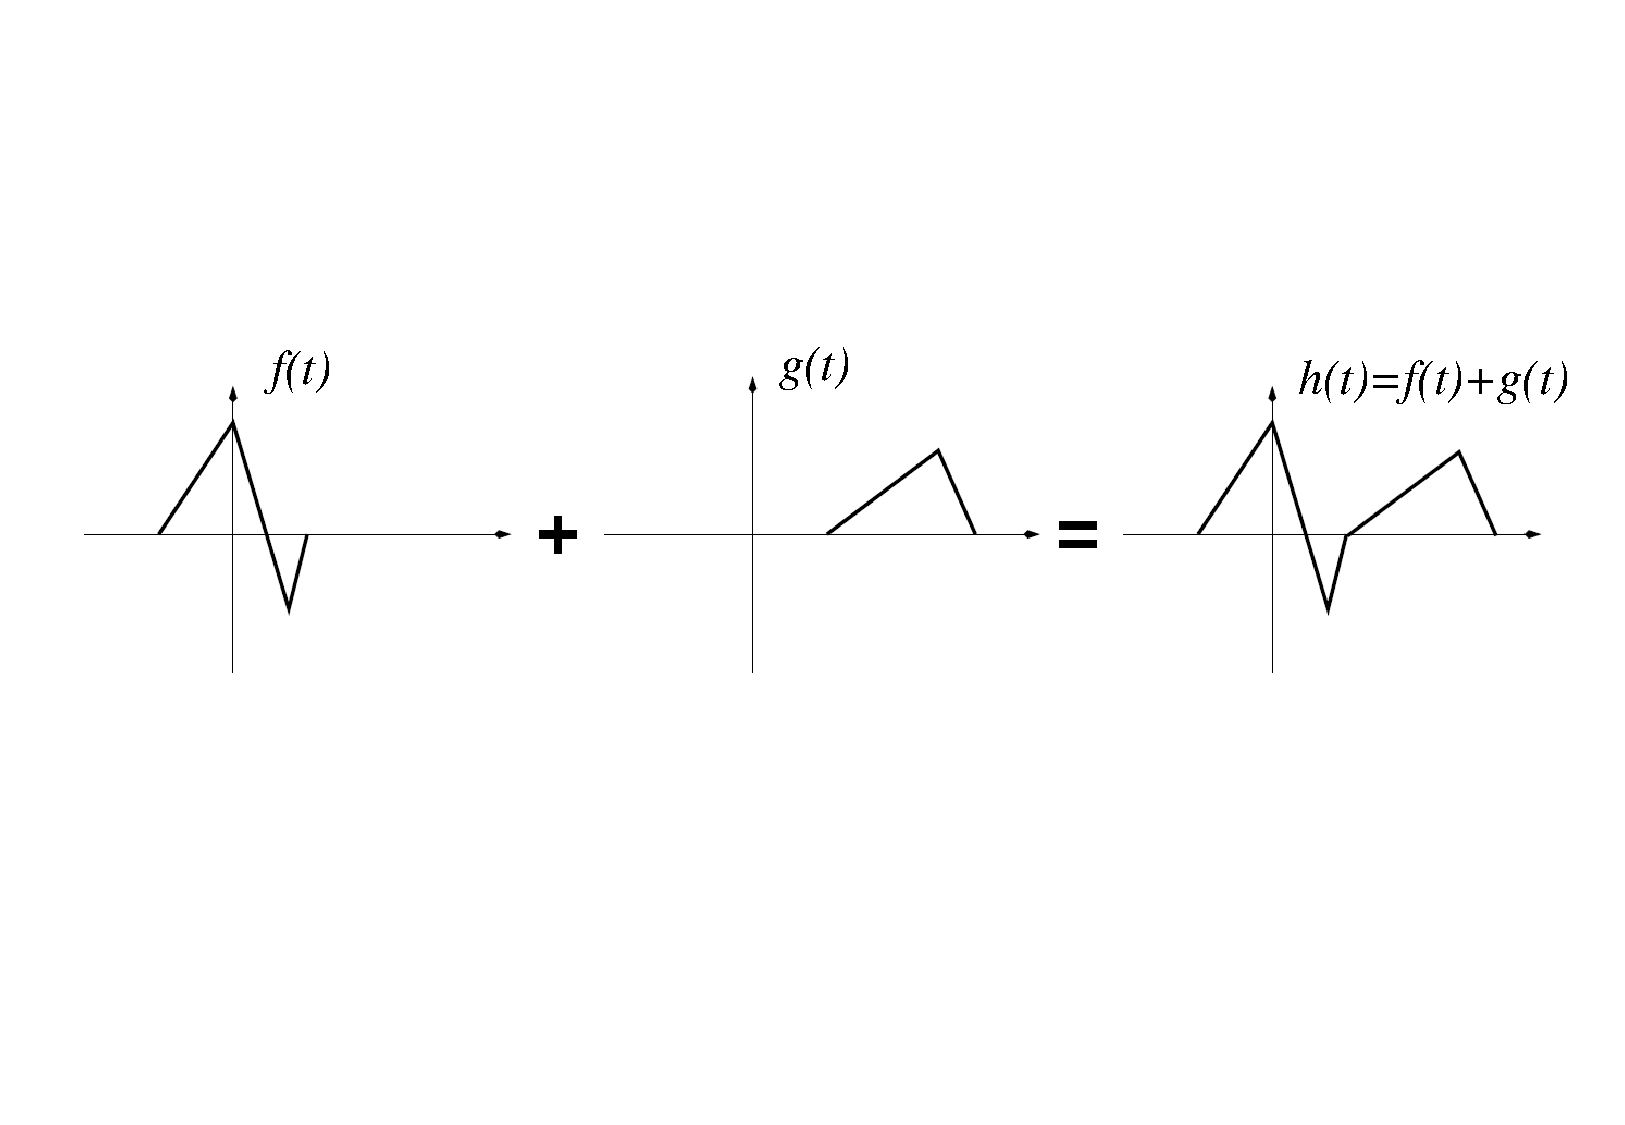
\includegraphics[width=1\textwidth]{img/op_somma_1.pdf}
		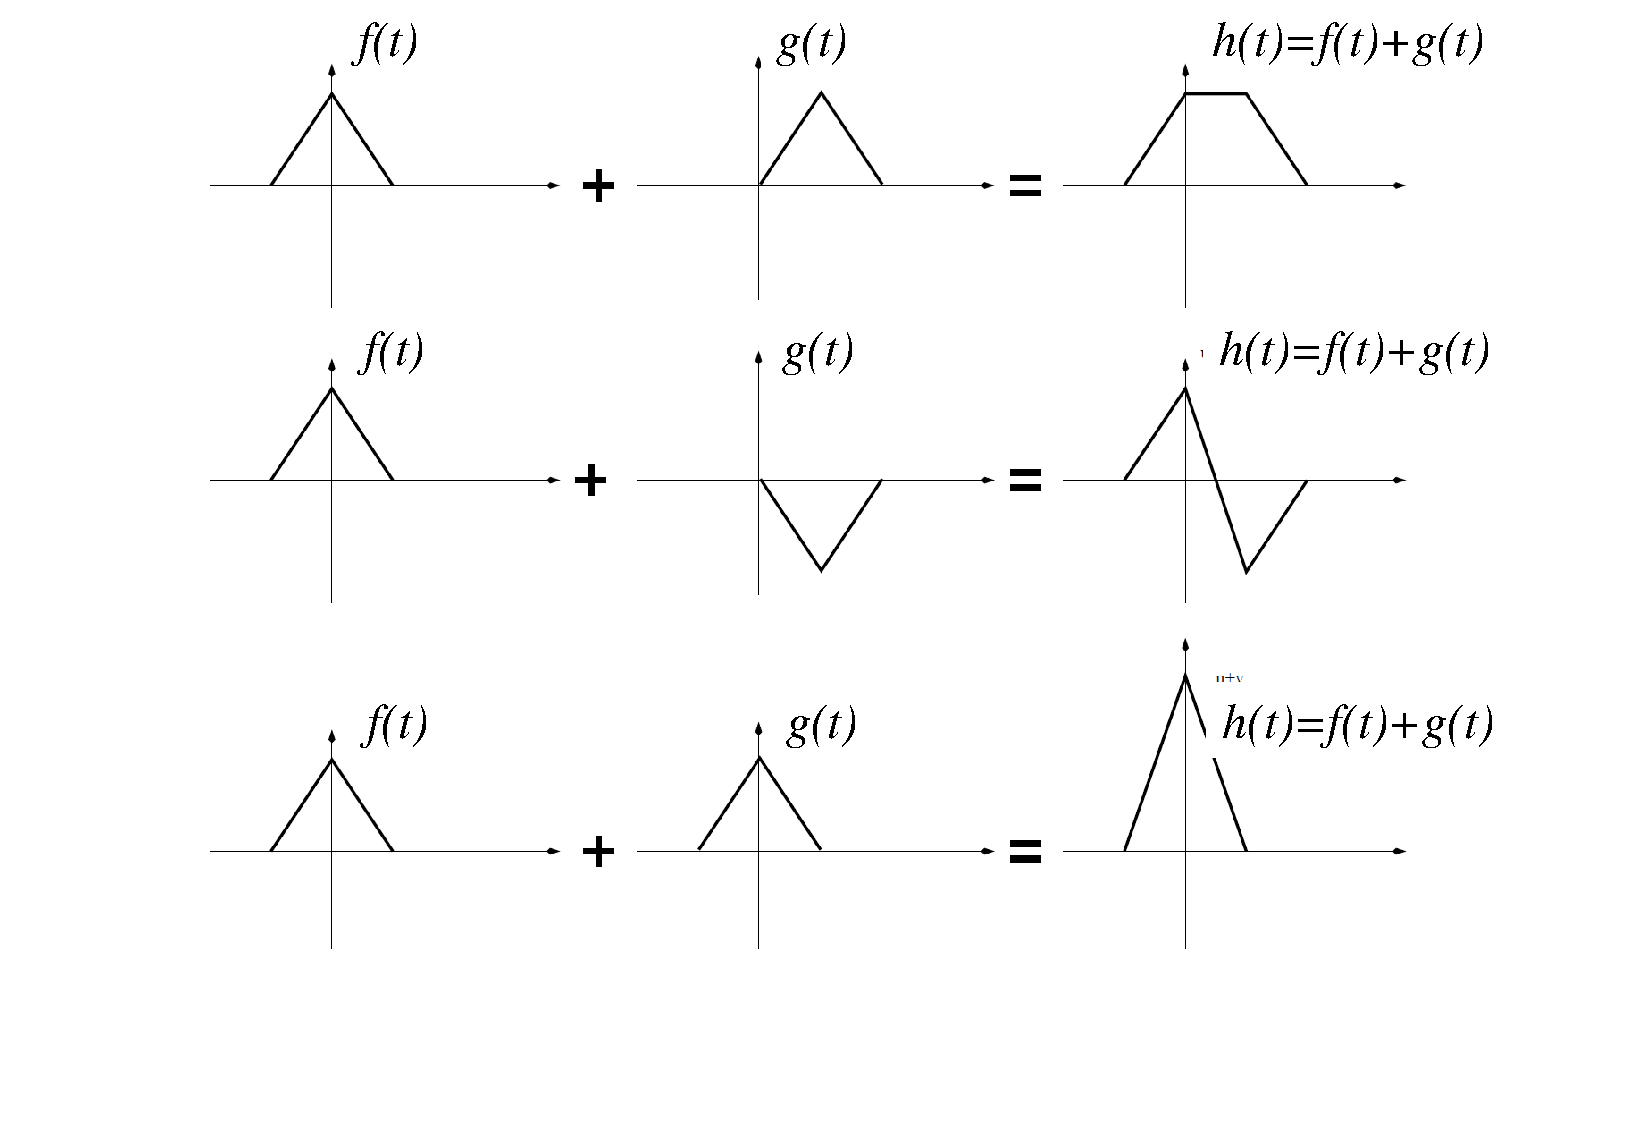
\includegraphics[width=1\textwidth]{img/op_somma_2.pdf}
	\end{figure}

	\newpage
	
	\subsubsection{Shift (o traslazione)}
	
	Lo \textbf{\emph{shift}} (o traslazione) è il cambio di posizione di un segnale. Può essere effettuato:
	
	\begin{itemize}
		\item \textbf{Traslazione a destra} con la funzione $f(t-\tau)$
		\item \textbf{Traslazione a sinistra} con la funzione $f(t+\tau)$
	\end{itemize}
	
	\begin{figure}[!htp]
		\centering
		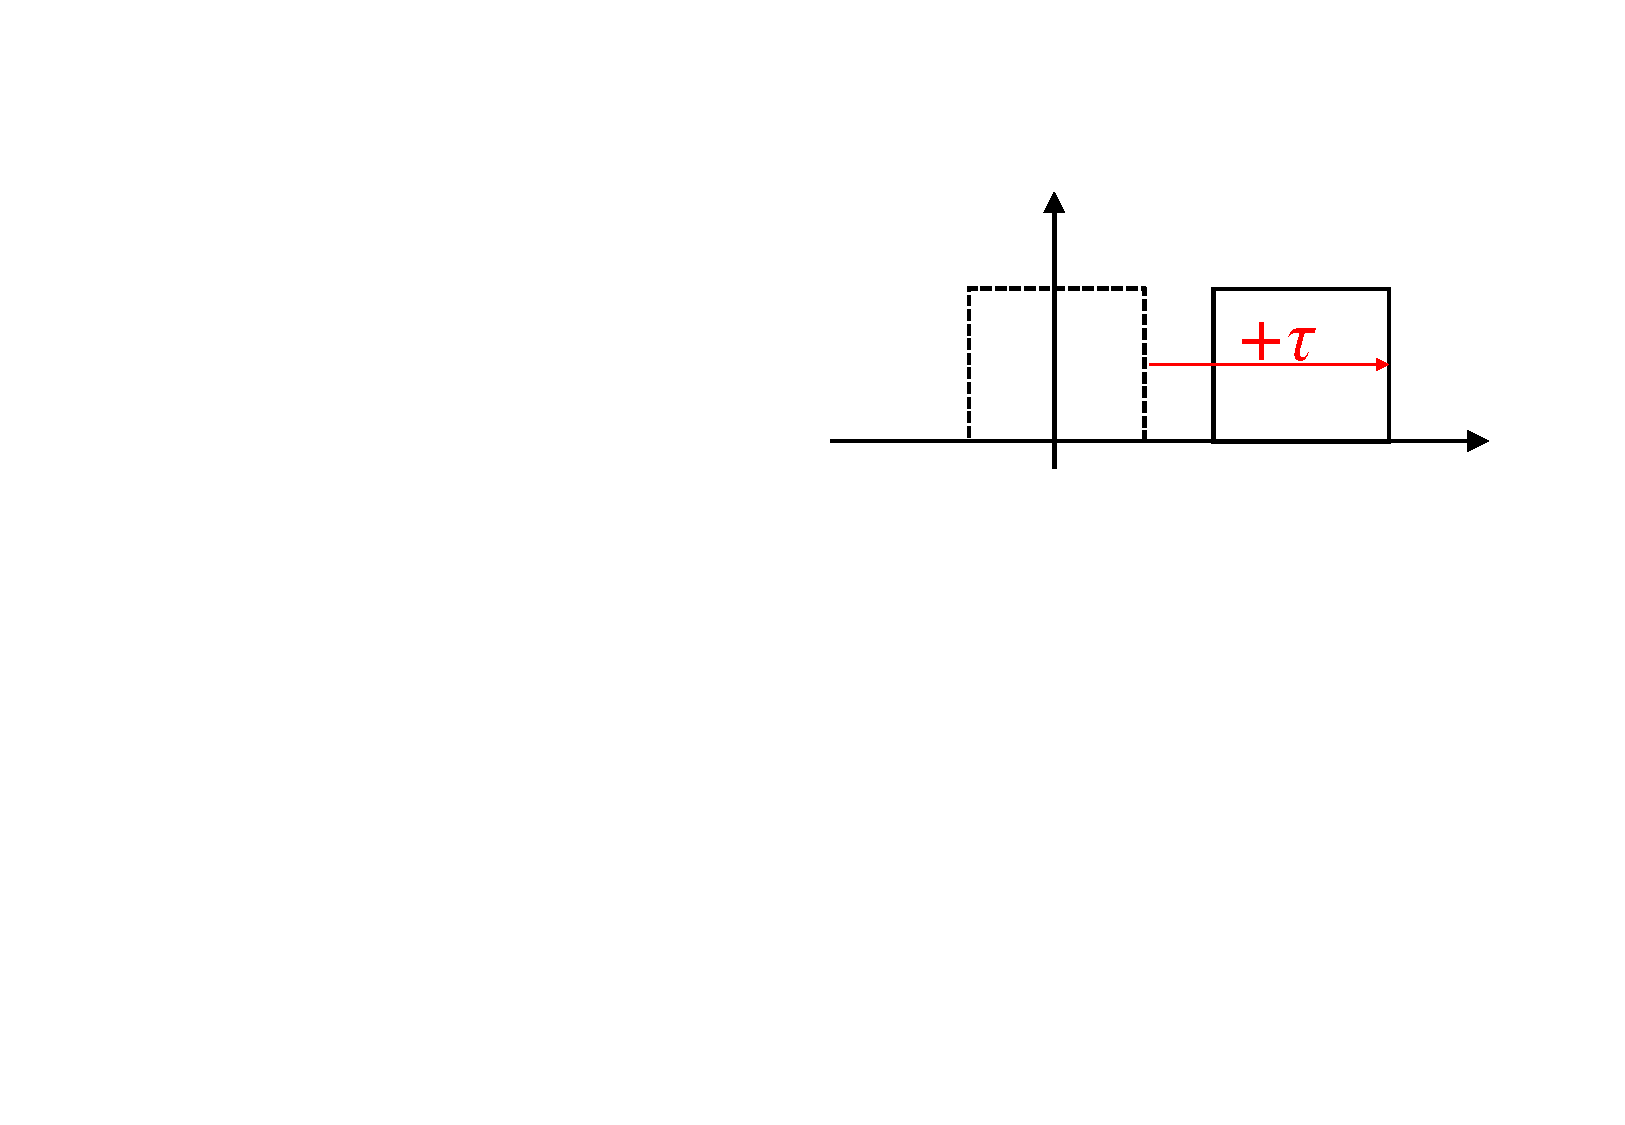
\includegraphics[width=0.5\textwidth]{img/op_shift_dx.pdf}\label{op_shift_dx}
		\caption{Shift a destra}
		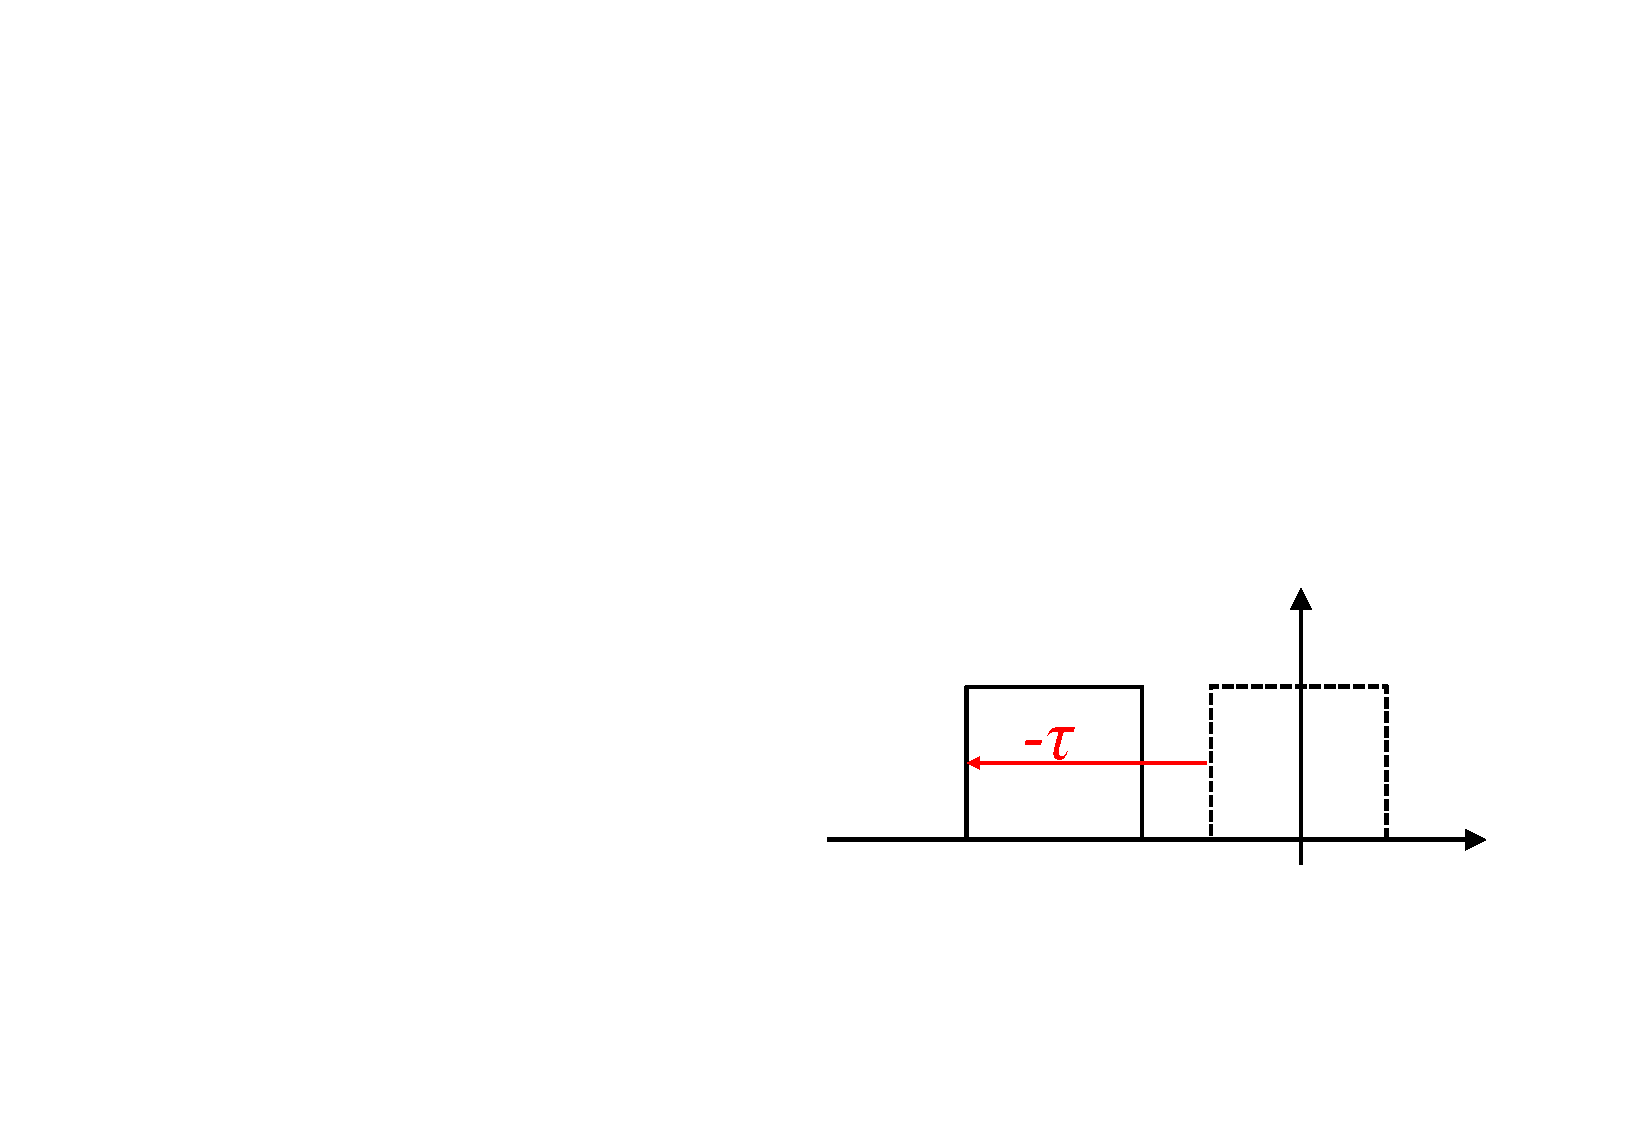
\includegraphics[width=0.5\textwidth]{img/op_shift_sx.pdf}\label{op_shift_sx}
		\caption{Shift a sinistra}
	\end{figure}

	\newpage
	
	\subsubsection{Funzione box $\Pi$ e impulso di Dirac}
	
	La funzione \textbf{\emph{box}} è definita nel seguente modo:
	
	\begin{equation*}
		A \Pi(\dfrac{x}{b}) \hspace{2em} x\in\left[-\dfrac{b}{2}, \dfrac{b}{2}\right]
	\end{equation*}

	\begin{figure}[!htp]
		\centering
		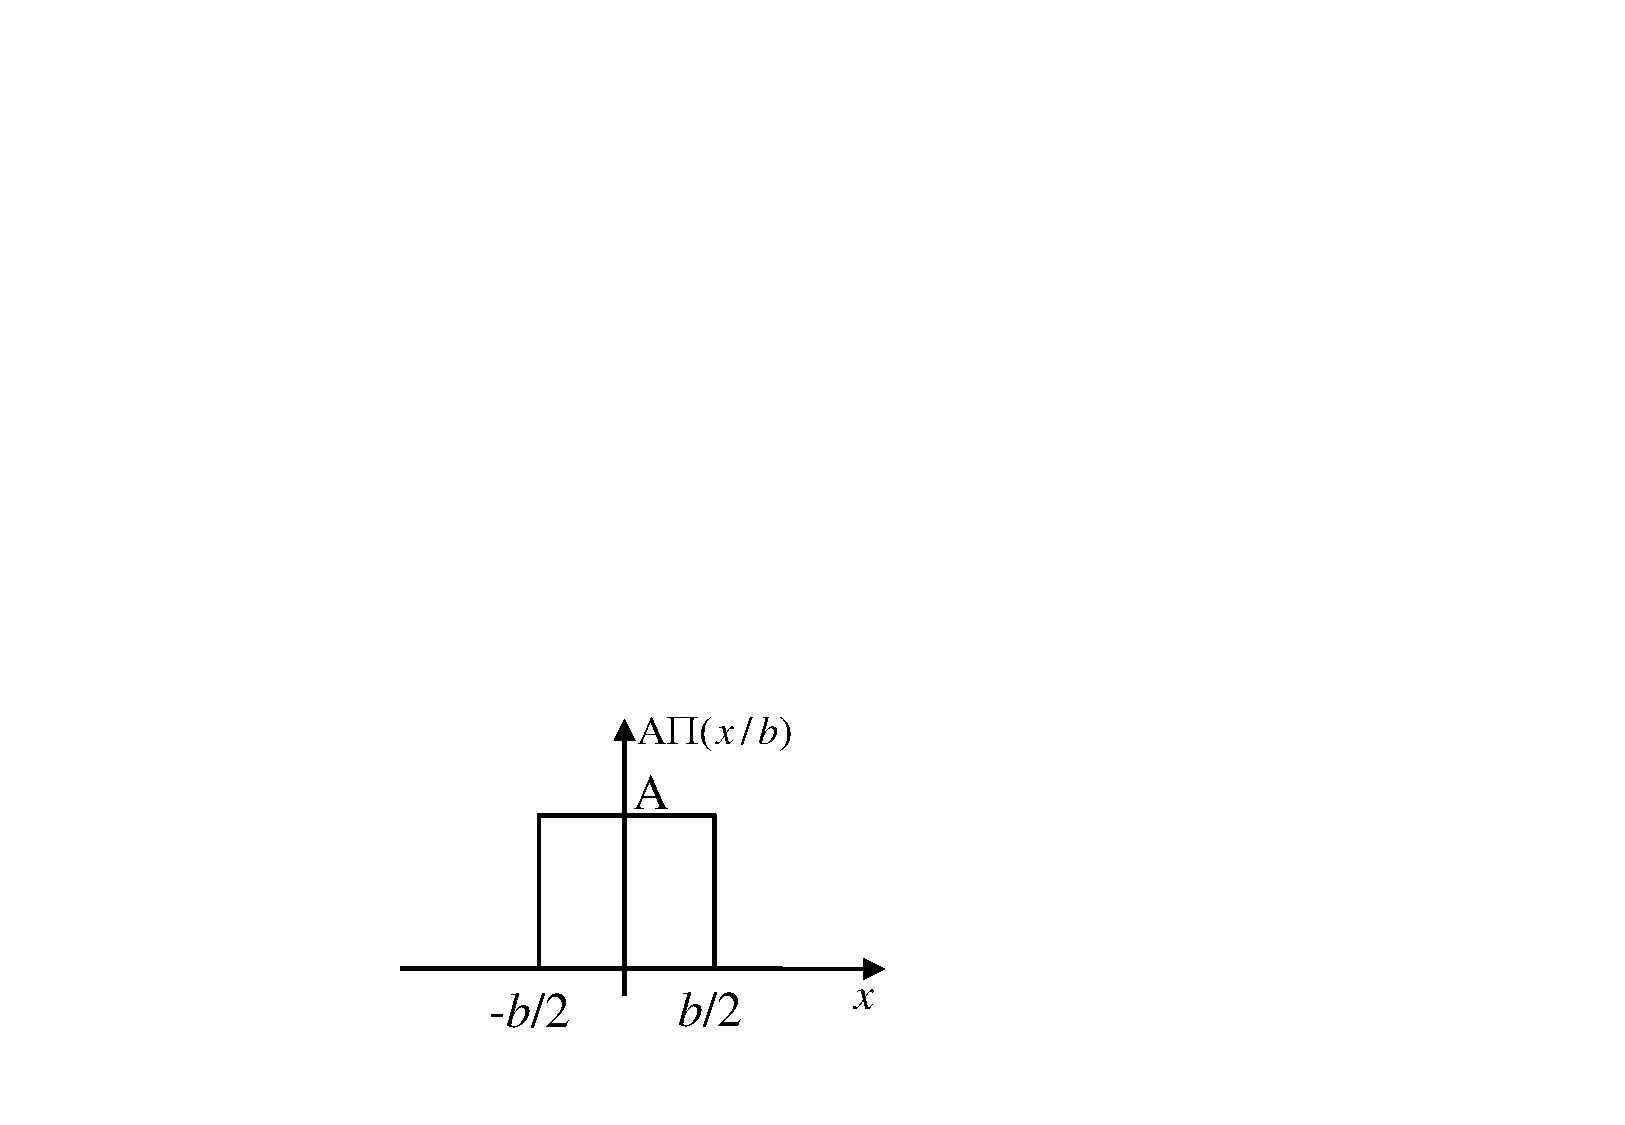
\includegraphics[width=0.4\textwidth]{img/box.pdf}\label{box}
		\caption{Box generica}
	\end{figure}

	La funzione $\delta(x)$ è chiamata \textbf{\emph{impulso unitario}} o \textbf{\emph{impulso di Dirac}} perché è definita nel seguente modo:
	
	\begin{equation*}
		\delta(x) = 
		\begin{cases}
			\infty  & \text{se } x=0 \\
			0		& \text{se } x\ne 0
		\end{cases}
		\hspace{2em} \int_{-\infty}^{\infty} \delta(x)\: dx = 1
	\end{equation*}

	\noindent
	Quindi è un impulso che tende all'infinito solamente quando la $x$ è nell'origine, ma il suo integrale è uguale a $1$. Alcune \textbf{proprietà} dell'impulso:
	
	\begin{enumerate}
		\item $\delta(x-x_0) = 0 \hspace{1em} \forall x\ne x_0$
		\item Data una funzione generica $f$ (\textbf{setacciamento}): $\displaystyle \int_{-\infty}^{\infty} f(x)\delta(x-x_0)\: dt = f(x_0)$
		\item $\delta(x - x_0) = \delta(x_0 - x)$
		\item $\delta(ax) = \dfrac{1}{|a|} \delta(x) \hspace{1em} \forall x \in \mathbb{R} \text{, fissato } a \in \mathbb{R}-\{0\}$
	\end{enumerate}

	\newpage
	
	\subsubsection{Funzione sinc}
	
	La funzione \textbf{\emph{sinc}} è definita nel seguente modo:
	
	\begin{equation*}
		\mathrm{sinc}(t) = \dfrac{\sin{\left(\pi t\right)}}{\pi t}
	\end{equation*}

	\noindent
	Ha due \textbf{caratteristiche} importanti: (1) l'intersezione con l'asse delle $x$ avviene sempre nei numeri interi positivi e negativi (quindi $1$ e $-1$, $2$ e $-2$, ecc.); (2) il limite $\displaystyle \lim_{t\rightarrow \pm\infty}\mathrm{sinc}(t) = 0$.\newline
	Questa funzione è \textbf{importante per l'analisi nel dominio del tempo} (o \textbf{frequenza}).
	
	\subsubsection{Funzione triangolo $\Lambda$}
	
	La funzione \textbf{\emph{triangolo}} è definita nel seguente modo:
	
	\begin{equation*}
		\Lambda(x) =
		\begin{cases}
			1-|x|, 	& |x| < 1 \\
			0		& \text{altrimenti}
		\end{cases}
	\end{equation*}

	\noindent
	Questa funzione è \textbf{importante per l'analisi spettrale e} per le \textbf{operazioni di convoluzione}.
	
	\subsubsection{Funzione segno ($sgn$)}
	
	La funzione \textbf{\emph{segno}} è definita nel seguente modo:
	
	\begin{equation*}
		\mathrm{sgn}(x) =
		\begin{cases}
			-1, 	& x < 0 \\
			+1,		& x > 0 \\
			0		& x = 0
		\end{cases}
	\end{equation*}
	
	\noindent
	Questa funzione ribalta segnali sopra o sotto l'asse delle $x$.
	
	\subsubsection{Funzione gradino}
	
	La funzione \textbf{\emph{gradino}} è definita nel seguente modo:
	
	\begin{equation*}
		u(x) =
		\begin{cases}
			0 & x < 0 \\
			1 & x \ge 0
		\end{cases}
	\end{equation*}
	
	\noindent
	Questa funzione rappresenta un \textbf{segnale} che si attiva a partire dal tempo specificato e rimane attivo indefinitamente. Attenzione! Non si confonda questo segnale con il segno.
	
	\newpage
	
	\subsubsection{Treno di impulsi}
	
	Il \textbf{\emph{treno di impulsi}} $S_{\Delta T}(x)$ è la somma di un numero infinito di impulsi periodici discreti distanziati di una quantità $\Delta T$:
	
	\begin{equation*}
		S_{\Delta T}(x) = \sum_{n = -\infty}^{\infty} \delta (x - n \Delta T) \hspace{1em} n \in \mathbb{Z}
	\end{equation*}

	\begin{figure}[!htp]
		\centering
		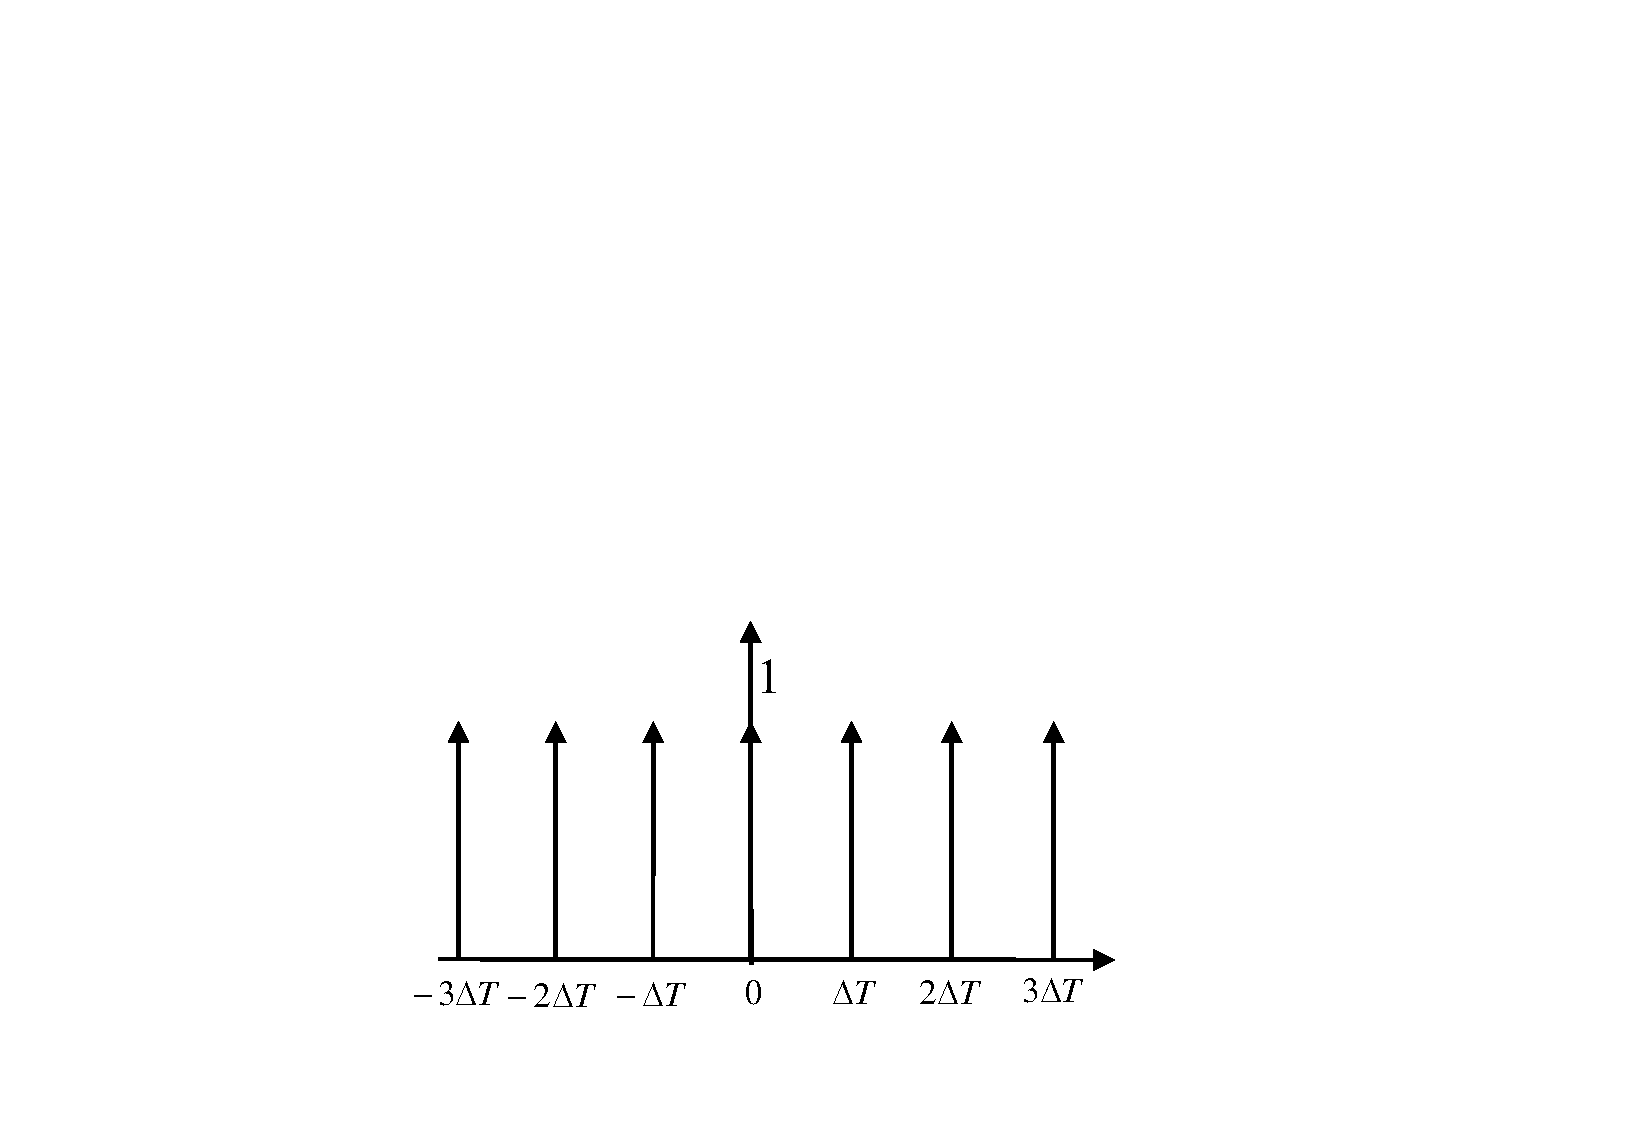
\includegraphics[width=0.5\textwidth]{img/treno_di_impulsi.pdf}\label{treno_di_impulsi}
		\caption{Treno di impulsi}
	\end{figure}

	\subsubsection{Energia di un segnale}
	
	L'\textbf{\emph{energia di un segnale}} è definita nel seguente modo:
	
	\begin{equation*}
		E_f =
		\begin{cases}
			\displaystyle \int_{-\infty}^{+\infty} f^{2}(t)\: dt & \text{se } f \in \mathbb{R} \\
			\displaystyle \int_{-\infty}^{+\infty} \left| f(t) \right|^{2} dt \hspace{1em} \text{con } \left| f(t) \right|^{2} = \tilde{f}(t) f(t), & f \in \mathbb{C}
		\end{cases}
	\end{equation*}
	
	\noindent
	Un segnale si dice \textbf{ad energia finita} (o \textbf{di energia}) se l'integrale che rappresenta l'energia converge ed è diverso da $0$. Quindi:
	
	\begin{itemize}
		\item[\ding{43}] \textbf{Condizione \emph{sufficiente}} all'esistenza della sua trasformata di Fourier. Le funzioni trigonometriche non sono di energia ma hanno comunque la Trasformata di Fourier.
		\item[\ding{42}] \textbf{Condizione \emph{necessaria}} per essere un segnale ad energia finita, all'infinito ($+\infty$ e $-\infty$) l'\textbf{ampiezza} va a zero.
	\end{itemize}

	\noindent
	Alcuni esempi:

	\begin{itemize}
		\item[\ding{80}] \textbf{Segnali di energia.} Impulsi rettangolari, oscillazioni smorzate ($\mathrm{sinc}$);
		\item[\ding{80}] \textbf{Segnali \underline{non} di energia.} Funzioni trigonometriche $\sin$ e $\cos$.
	\end{itemize}

	\noindent
	L'\textbf{unità di misura} è il \emph{joule}.
	
	\subsubsection{Potenza media di un segnale}
	
	La \textbf{\emph{potenza media di un segnale}} è definita nel seguente modo:
	
	\begin{equation*}
		P_f =
		\begin{cases}
			\displaystyle \lim_{T \rightarrow +\infty} \dfrac{1}{T} \int_{-\dfrac{T}{2}}^{+\dfrac{T}{2}} f^{2}(t)\: dt & \text{se } f \in \mathbb{R} \\
			\displaystyle \lim_{T \rightarrow +\infty} \dfrac{1}{T} \int_{-\dfrac{T}{2}}^{+\dfrac{T}{2}} \left|f(t)\right|^{2}\: dt \hspace{1em} \text{con } \left| f(t) \right|^{2} = \tilde{f}(t) f(t), & f \in \mathbb{C}
		\end{cases}
	\end{equation*}
	
	\noindent
	Un segnale si dice \textbf{a potenza finita} (o \textbf{di potenza}) se l'integrale che rappresenta la potenza converge ed è diverso da $0$. L'\textbf{unità di misura} è il \emph{watt}.\newline
	Infine, un segnale ad energia finita ha la potenza che tende a zero (per cui un segnale non può appartenere ad entrambe le categorie). Invece, esistono segnali che non sono né di energia, n* di potenza finita.
	
	\newpage
	
	\subsection{Altre operazioni fondamentali}
	
	\subsubsection{Rescaling (o riscalatura)}
	
	La funzione di \textbf{\emph{rescaling}} è definita nel seguente modo:
	
	\begin{equation*}
		\forall f(t) : D_1 \in \mathbb{R}, \hspace{1em} \omega \ne 0
	\end{equation*}
	
	\noindent
	Simile allo \emph{shift}, il \emph{rescaling} ha una definizione generica e due varianti:
	
	\begin{itemize}
		\item \textbf{Definizione generica} con la funzione semplice $f(t)$ (immagine~\ref{rescaling}).
		\item \textbf{Ritardo \underline{lineare} del segnale di un fattore $\omega$} con la funzione $f(\omega t), 0 < \omega < 1$ (immagine~\ref{rescaling_ritardo}).
		\item \textbf{Accelero \underline{lineare} del segnale di un fattore $\omega$} con la funzione $f(\omega t), \omega > 1$ (immagine~\ref{rescaling_accelero}).
	\end{itemize}
	
	\begin{figure}[!htp]
		\centering
		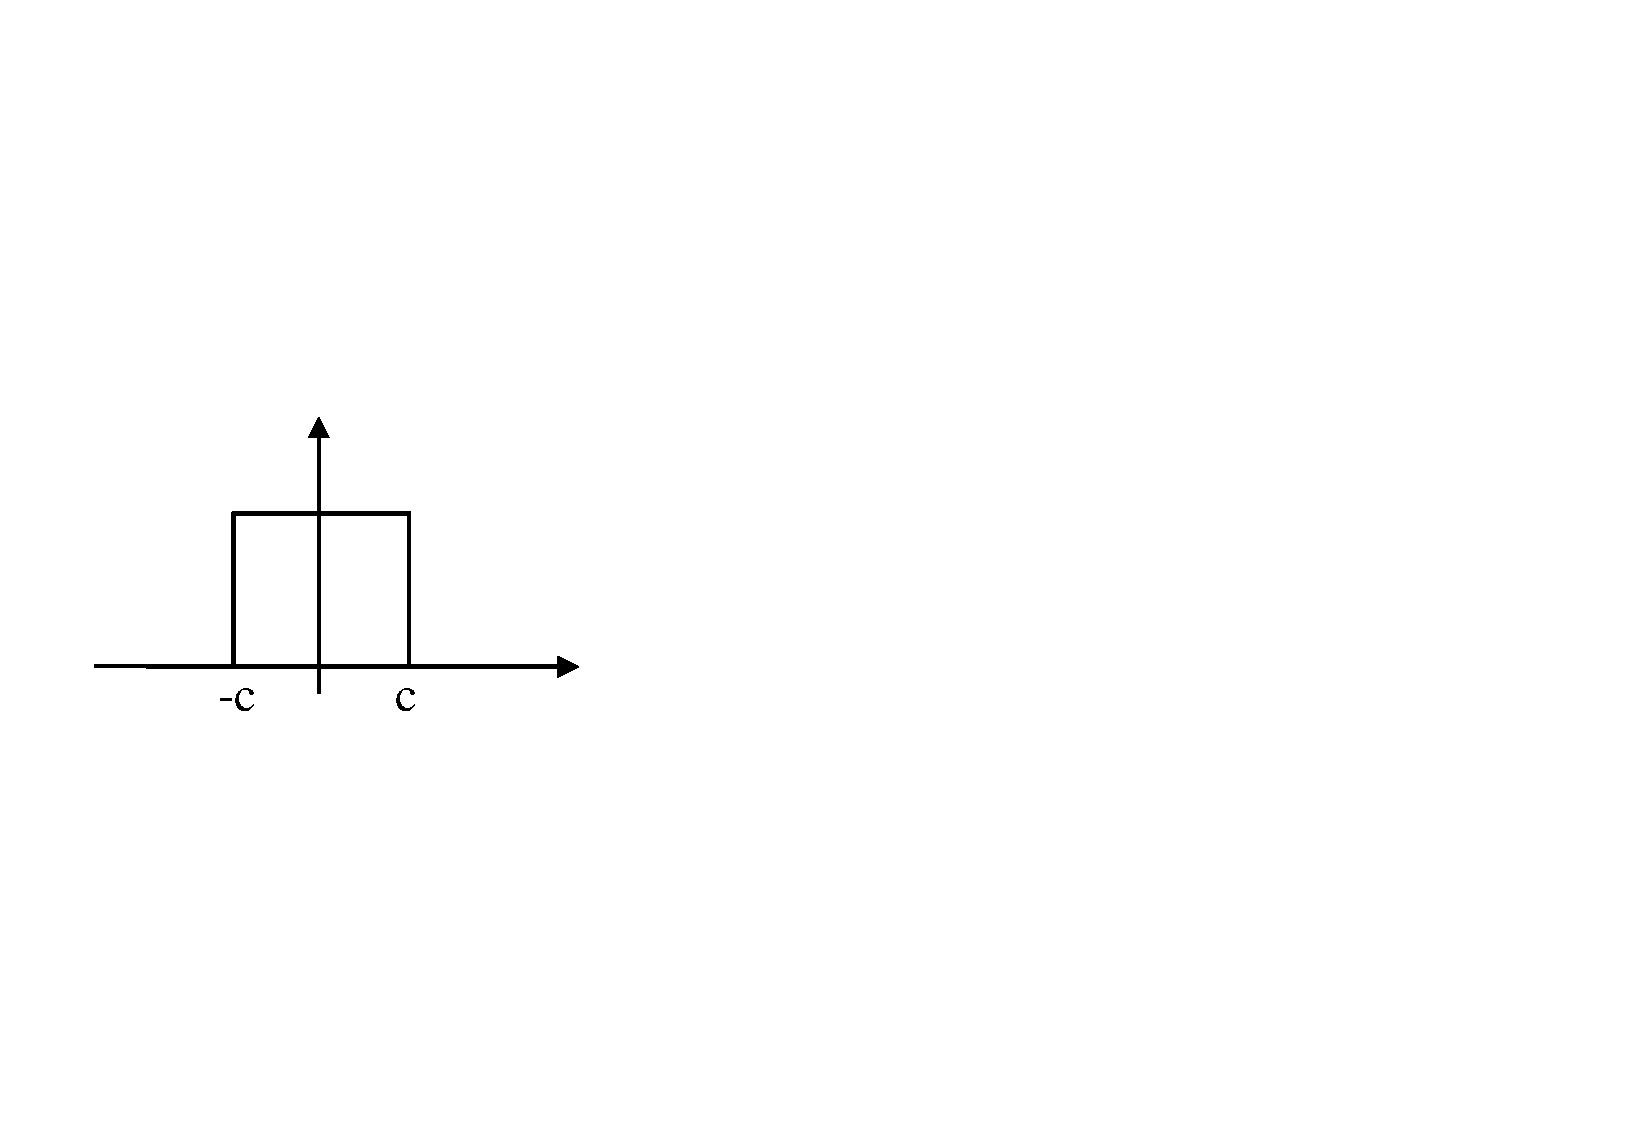
\includegraphics[width=0.5\textwidth]{img/rescaling.pdf}\label{rescaling}
		\caption{Definizione generica}
		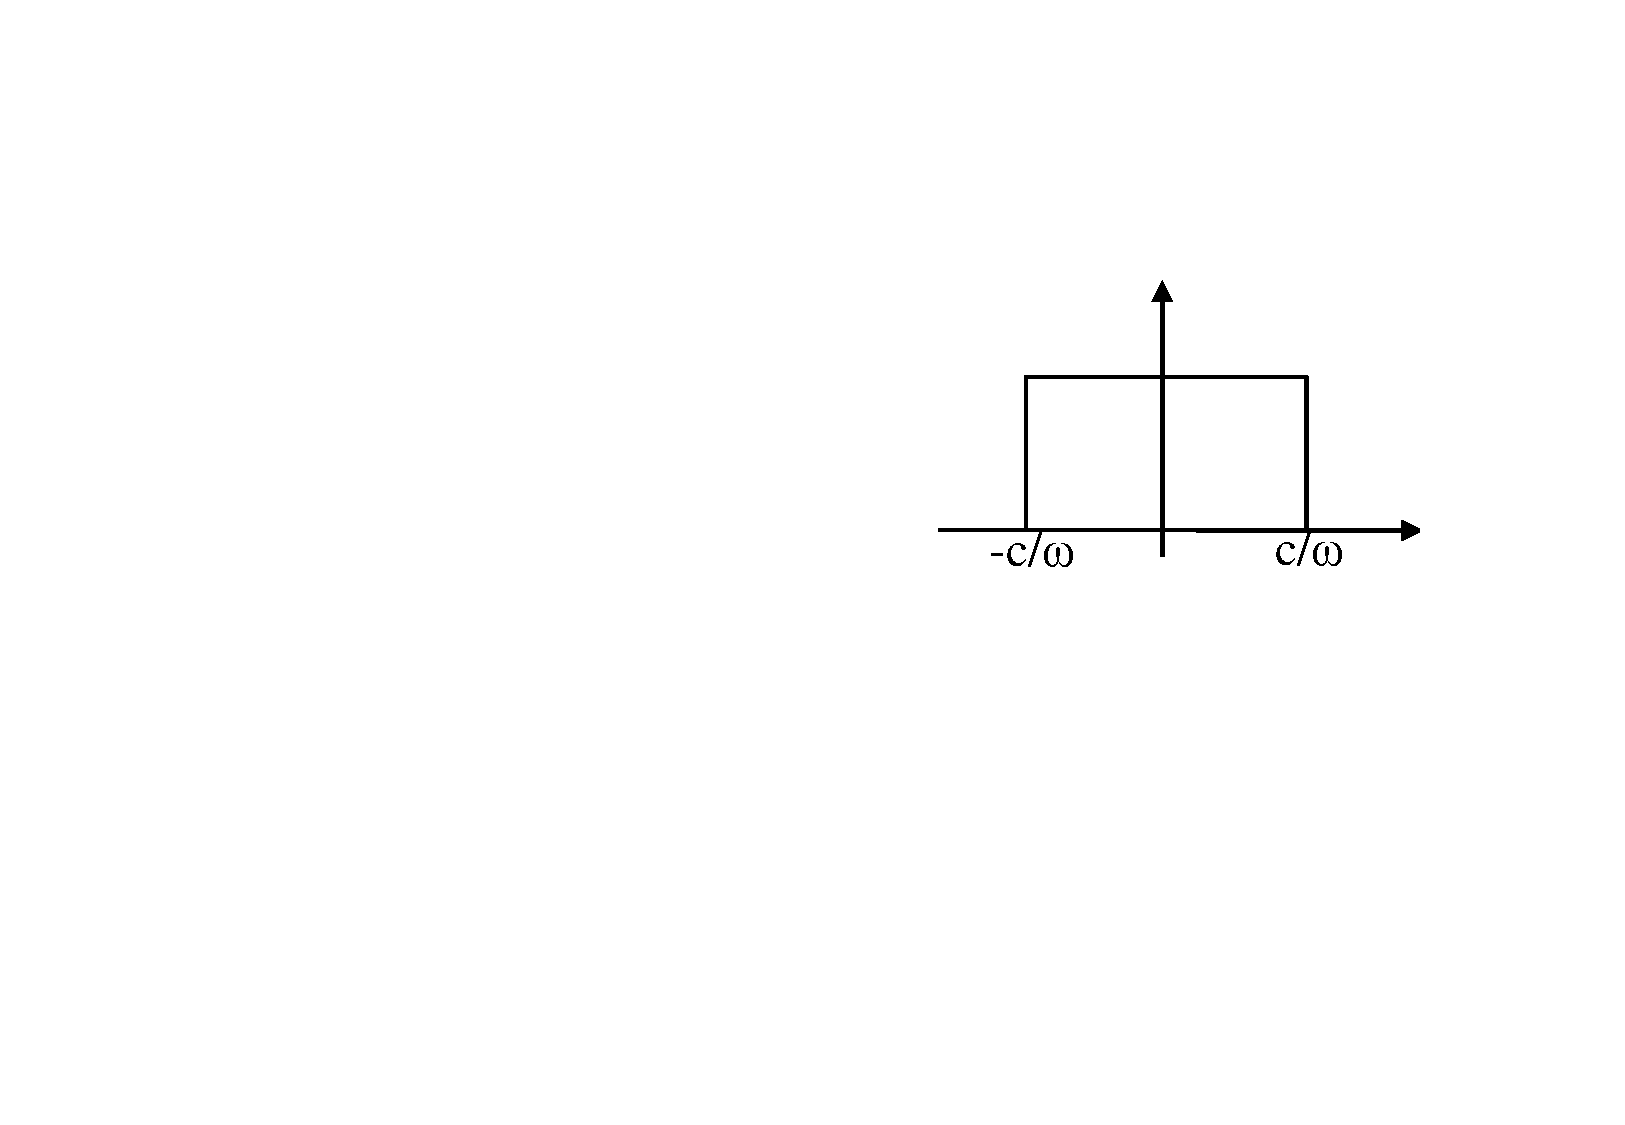
\includegraphics[width=0.5\textwidth]{img/rescaling_ritardo.pdf}\label{rescaling_ritardo}
		\caption{Ritardo \underline{lineare} del segnale di un fattore $\omega$}
		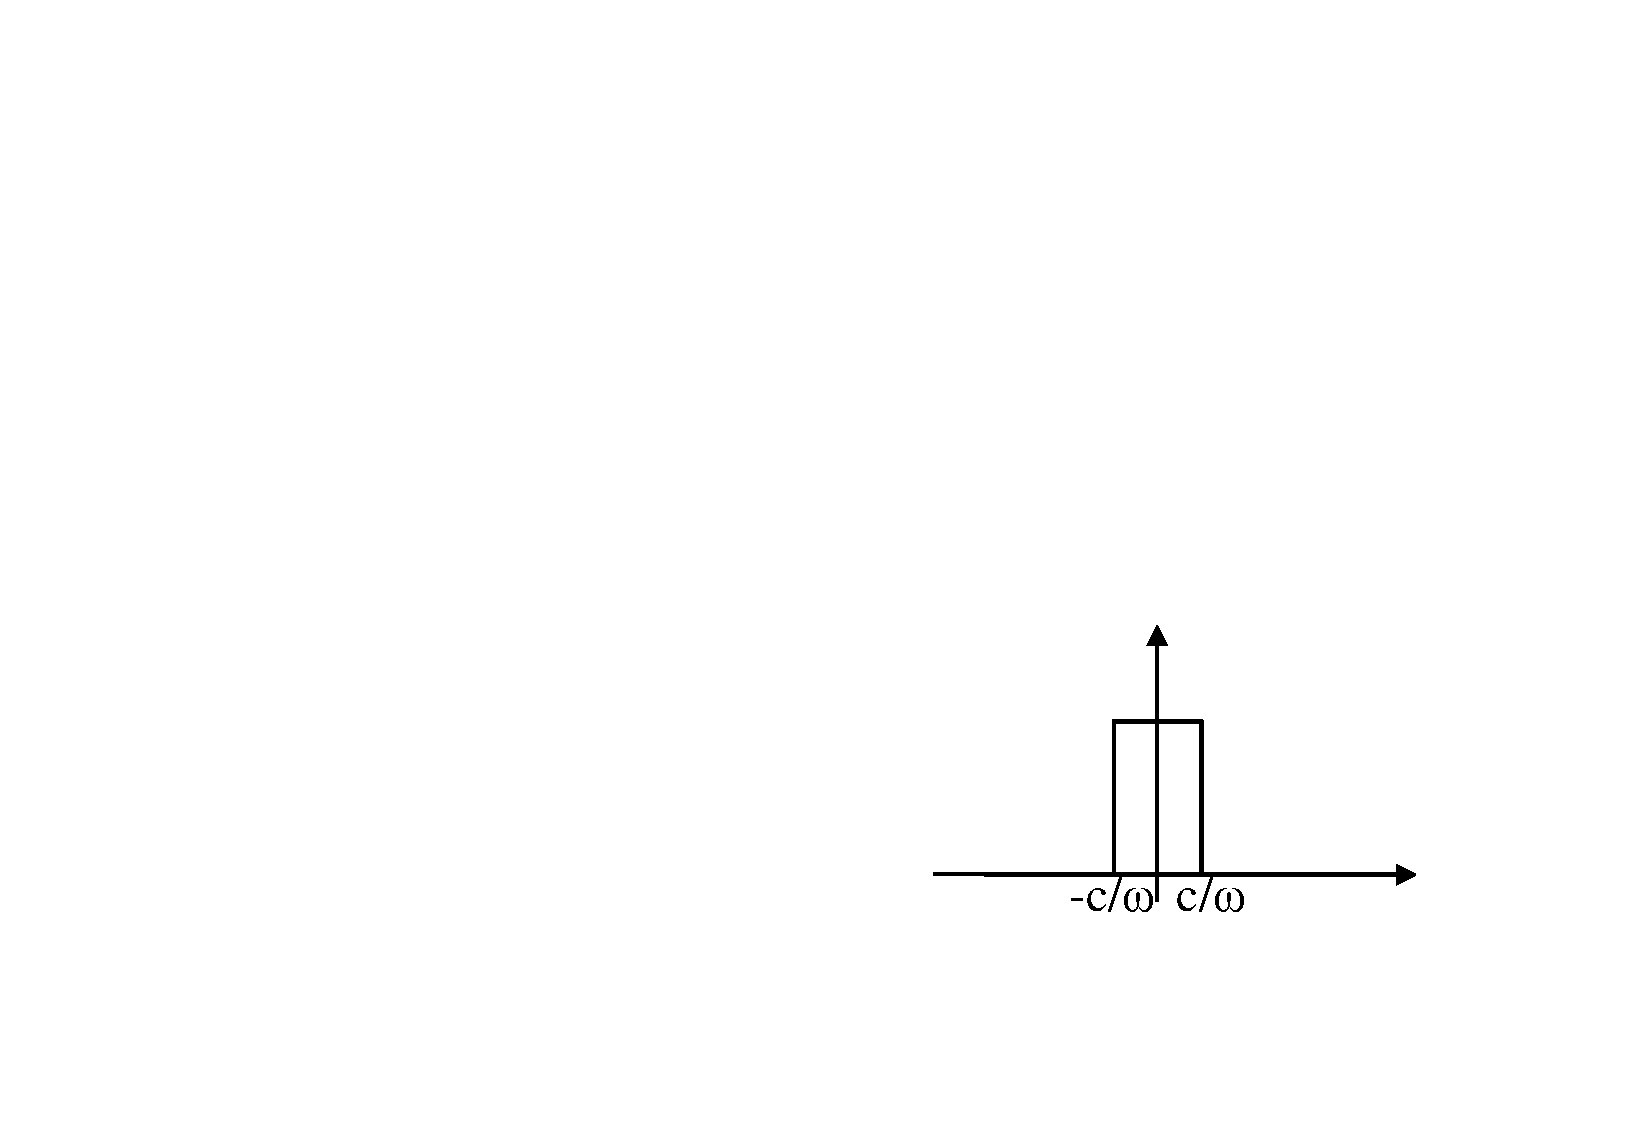
\includegraphics[width=0.5\textwidth]{img/rescaling_accelero.pdf}\label{rescaling_accelero}
		\caption{Accelero \underline{lineare} del segnale di un fattore $\omega$}
	\end{figure}

	\subsubsection{Cross-Correlazione}
	
	Dati $f_1(\tau), f_2(\tau)$ segnali continui, $\tau\in\mathbb{R}$ il segnale di \textbf{\emph{cross-correlazione}} viene definito come:
	
	\begin{equation*}
		\displaystyle f_1 \otimes f_2 (t) = \int_{-\infty}^{+\infty} \tilde{f_1}(\tau) f_2(\tau - t)\: d\tau
	\end{equation*}

	\noindent
	In cui $\tilde{f_1}(\tau)$ rappresenta un \emph{complesso coniugato}. Nel caso in cui $f_1$ è reale, allora $\tilde{f_1}(\tau) \rightarrow f_1(\tau)$. \newline
	Infine, con $t = 0$ si ha l'\textbf{\emph{integrale di cross-correlazione}}, il quale è definito se l'integrale converge (ovviamente se il segnale non è né di energia, né di potenza, la convergenza non esiste!).
\end{document}